\begin{figure}[t]
\centering
\begin{subfigure}[t]{0.4\textwidth}
\centering
\begin{tikzpicture}[scale=0.75,transform shape]
\GraphInit[vstyle=Classic]
\SetGraphUnit{2.5}
\Vertex[x=3,y=0]{A}
\Vertex[x=3,y=3]{B}
\Vertex[x=0,y=3,Lpos=180]{C}
\tikzset{VertexStyle/.style = {
shape = circle,
fill = white,
inner sep = 0pt,
outer sep = 0pt,
minimum size = 12pt,
draw}}
\Vertex[x=0,y=0,Lpos=180]{S}
\Edge[label=$2$](S)(C)
\Edge[label=$3$](S)(A)
\Edge[label=$1$](C)(B)
\Edge[label=$5$](C)(A)
\end{tikzpicture}
\caption{}
\end{subfigure}
\;
\begin{subfigure}[t]{0.4\textwidth}
\centering
\begin{tikzpicture}[scale=0.75,transform shape]
\GraphInit[vstyle=Classic]
\SetGraphUnit{2.5}
\Vertex[x=3,y=0]{A}
\Vertex[x=3,y=3]{B}
\tikzset{VertexStyle/.style = {
shape = circle,
fill = white,
inner sep = 0pt,
outer sep = 0pt,
minimum size = 12pt,
draw}}
\Vertex[x=0,y=0,Lpos=180]{S}
\Vertex[x=0,y=3,Lpos=180]{C}
\Edge[local,label=$2$,color=blue](S)(C)
\Edge[label=$3$](S)(A)
\Edge[label=$1$](C)(B)
\Edge[label=$5$](C)(A)
\end{tikzpicture}
\caption{}
\end{subfigure}

\vspace{10pt}
\begin{subfigure}[t]{0.4\textwidth}
\centering
\begin{tikzpicture}[scale=0.75,transform shape]
\GraphInit[vstyle=Classic]
\SetGraphUnit{2.5}
\Vertex[x=3,y=0]{A}
\tikzset{VertexStyle/.style = {
shape = circle,
fill = white,
inner sep = 0pt,
outer sep = 0pt,
minimum size = 12pt,
draw}}
\Vertex[x=0,y=0,Lpos=180]{S}
\Vertex[x=0,y=3,Lpos=180]{C}
\Vertex[x=3,y=3]{B}
\Edge[local,label=$2$,color=blue](S)(C)
\Edge[local,label=$1$,color=blue](C)(B)
\Edge[label=$3$](S)(A)
\Edge[label=$5$](C)(A)
\end{tikzpicture}
\caption{}
\end{subfigure}
\;
\begin{subfigure}[t]{0.4\textwidth}
\centering
\begin{tikzpicture}[scale=0.75,transform shape]
\GraphInit[vstyle=Classic]
\SetGraphUnit{2.5}
\tikzset{VertexStyle/.style = {
shape = circle,
fill = white,
inner sep = 0pt,
outer sep = 0pt,
minimum size = 12pt,
draw}}
\Vertex[x=0,y=0,Lpos=180]{S}
\Vertex[x=0,y=3,Lpos=180]{C}
\Vertex[x=3,y=3]{B}
\Vertex[x=3,y=0]{A}
\Edge[local,label=$2$,color=blue](S)(C)
\Edge[local,label=$1$,color=blue](C)(B)
\Edge[local,label=$3$,color=blue](S)(A)
\Edge[label=$5$](C)(A)
\end{tikzpicture}
\caption{}
\end{subfigure}
\caption{The execution of Prim's algorithm on a weighted graph $G$ with 4
vertices. White vertices represent elements of $X$, while black vertices
represent elements of $V - X$. Blue edges represent edges added to the
output spanning tree $T^*$. In step (a), the inital element $S \in X$ is
chosen arbitrarily. We see that in step (d), Prim's algorithm halts as $X = V$
and $T^*$ is indeed a minimum spanning tree of $G$.}
\label{fig:prim-example}
\end{figure}

